
Face Generation is an important field in the market, it is used widely in all camera applications to apply filters on the taken images most of the usage was for entertainment, Although it can be used to have photos for any missing people or criminal and that will increase the chance to find that missing people or the criminal.
 
\subsection{Targeted Customers}
Our Project is directed to all governmental and volunteering organizations, that need to generate identical faces of missing people from bare human description of their facial features.
It also can be used to identify the ancient kings and queens faces from the Papyrus .
We can categorize the different target companies into the following:
\begin{itemize}
    \item \textbf{Criminal identification from witnesses descriptions :}
        \begin{itemize}
            \item INTERPOL.
            \item Different Police Stations.
        \end{itemize}
    \item \textbf{Missing People organizations like :}
        \begin{itemize}
            \item International Center for Missing and Exploited Children.
            \item International Red Cross and Red Crescent Movement.
            \item International Commission on Missing Persons \emph{ICMP}
            \item The Doe Network.
            \item National Missing and Unidentified Persons System.
            \item Missing Persons Support Center.
            \item LostMissing Inc.
            \item Missing People In America.
            \item Be United Missing Persons Inc.
            \item others.
        \end{itemize}
    \item \textbf{Historical Characters Identification :}
        \begin{itemize}
            \item Archaeological and Historical Research Facilities.
        \end{itemize}
\end{itemize}

\subsection{Market Survey}

As mentioned previously, most Applications that uses face generation is for entertainment, So they depends only on image refinement on limited number of features to generate the image unlike us, We have both image generation and refinement using 34 features for generation and 38 for refinement.
Besides that our goal is to find missing person for purpose more important than entertaining. Our biggest competitor is FaceApp, followed by PicsArt, Facetune2 and Booth Apps.
  

\subsubsection{FaceAPP}

\begin{figure}[H]
    \centering
    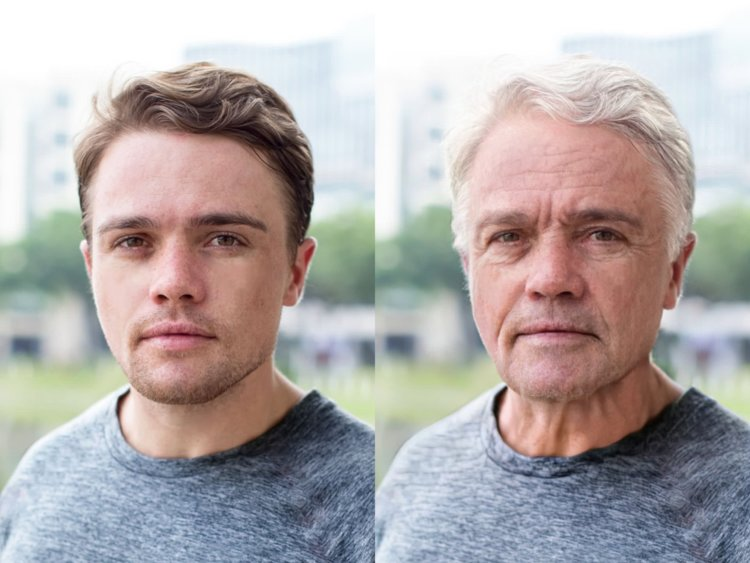
\includegraphics[width=0.6\textwidth]{images/FaceApp.jpg}
    \caption{Changing Age using FaceApp application.}
    \label{fig:faceApp}
\end{figure}

\emph{FaceAPP} is considered Image and video editing mobile application, it generates highly realistic transformations of human faces in photographs using AI and Neural Networks. 
The Limitation of the App compared with us, it only used for refinement using 14 facial feature which may be not enough for generating face from scratch.

\subsubsection{PicsArt}

\begin{figure}[H]
    \centering
    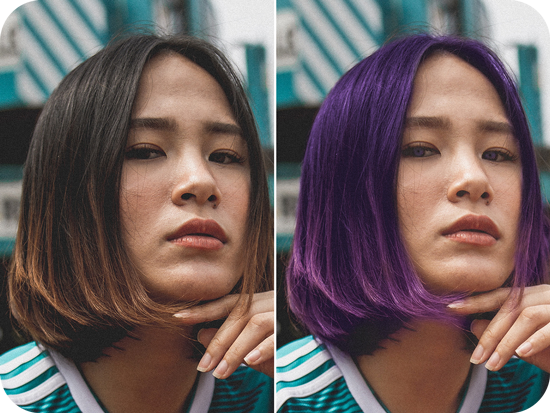
\includegraphics[width=0.6\textwidth]{images/picsArt.png}
    \caption{image refinement using PicsArt application.}
    \label{fig:picsArt}
\end{figure}

\emph{PicsArt} is a company that develops online photo and video editing applications, with a social creative community. The platform allows users to take and edit pictures and videos and draw with layers. It only allows 9 features refinement so it's also not the best choice for image generation.

\subsubsection{Facetune2}

\begin{figure}[H]
    \centering
    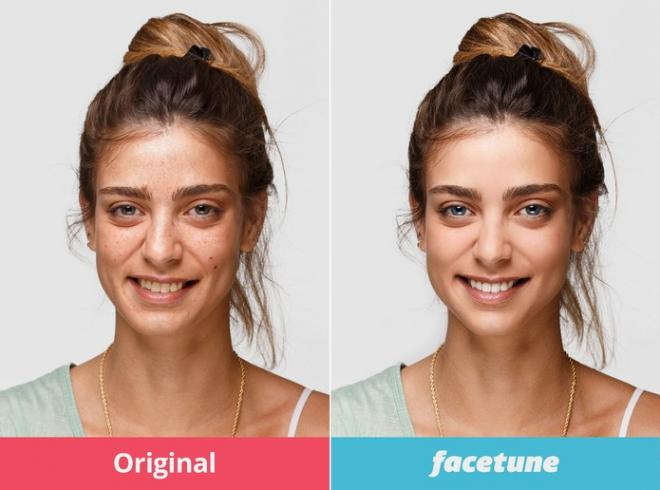
\includegraphics[width=0.5\textwidth]{images/FaceTune.jpg}
    \caption{image refinement using FaceTune2 application.}
    \label{fig:FaceTune2}
\end{figure}

\emph{Facetune2} is a photo editing application. It's commonly used to enhance the portrait o selfie images and offers 7 feature refinements.

\subsubsection{Booth Apps}

\begin{figure}[H]
    \centering
    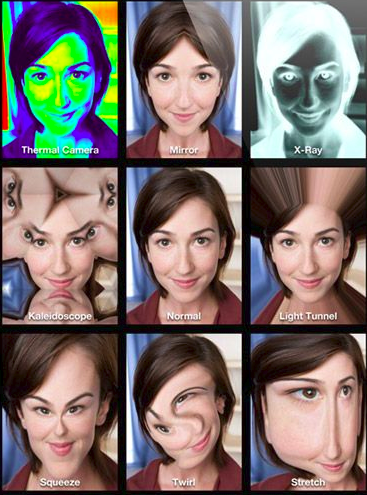
\includegraphics[width=0.5\textwidth]{images/photoBooth.png}
    \caption{image Editing using PhotoBooth application.}
    \label{fig:photoBooth}
\end{figure}

\emph{Booth Apps} are a collection of applications for image or video editing and enhancement, can add animation to an image and many other entertaining features. Examples for Booth Apps are : Simple Booth Classic, Mini Photobooth, Pocketbooth, Photobooth mini and My Photobooth App.
They only consider image enhancement and for entertaining purposes not critical issues like our product.

\subsection{Business Case and Financial Analysis }

Our product is new in the market which makes our business case a good one. We can provide our services in two forms as following:
\begin{itemize}
    \item The first is being a software service that is used in police stations so that any missing people or theft happens, they enters the description of that person so they can have an image for him/her to be able to find him faster, Or used in historical institutions that is responsible for finding information about the history from papyrus.
    \item The second one is a website for general users to be able to use it to generate images for their ancestors who died without having any images, from their parents' descriptions so they can see them, or for any entertaining purposes.
\end{itemize}

The financial analysis of this application is done after detailed market research.
The cost estimation for our software as a service in a specific institution is the cost behind the hardware, our application takes around 1 second on an \emph{Nvidia GTX 1080 ti} for generating the face from any description, but this can extend to be multiple seconds based on the connection. The whole system can be deployed on single PC with 11GB VRAM, around 700\$ for the GPU and 1500\$ to 2000\$ for the whole PC. For scalability, we can use 2 PCs one for generation and the other for Pose estimation to host the whole application. Also, we can scale out our system on more than 2 PCs for improved request parallelism. For the second type of usage we can deploy the system on cloud instance which costs around 150\$ per month for these specifications.
